% !TEX root =  paper.tex
\section{Evaluation}
\label{sec:evaluation}
To evaluate \toolname, we conducted qualitative and quantitative studies  
to answer the following research questions:

\begin{enumerate}[label=\textbf{RQ\arabic*},leftmargin=*]
	\item How accurate is \toolname in inferring semantic groupings and semantic roles?

	\item To what extent can \toolname detect accessibility failures 
    in real-world web pages?
\end{enumerate}

In the following subsections, we discuss the details of the experiments that 
we designed to answer each research question, together with the results.

\subsection{RQ1: Semantic Grouping and Roles Inference}
In this question, the objective is to assess how accurate the semantic grouping and semantic role inference processes are. 
The rationale for evaluating this aspect is that the approach 
first performs the grouping and semantics inference, and then 
uses this inference to test for accessibility. Accordingly, 
we first need to assess the inference process itself. 

We evaluated this question as follows. 
First, we collected 10 random subjects from the Moz 
Top 500~\footnote{https://moz.com/top500} most popular websites. 
Our approach does not have specific requirements for a subject other 
than being able to load it in a browser and access its DOM.  
We then ran the approach on each test subject's URL and obtained 
the output groupings and semantic roles. 
\Cref{fig:output} shows an example of the output. 
Each rectangle represents an inferred grouping, together 
with its semantic role. 
Subsequently, we recruited human evaluators. 
10 evaluators were recruited from the MTurk~\footnote{https://www.mturk.com} 
crowdsourcing platform. The qualifications of participants 
are to be working in the software industry and to have maintained the 
highest level of accuracy on the MTurk platform, which is referred to 
as Masters level.

Subsequently, each human evaluator was presented with the output of \toolname 
for all test subjects, and asked to assess the accuracy of groupings and roles.  
More specifically, we asked them to identify any output groups 
that do not represent a meaningful semantic grouping. This represents 
the \emph{false positives} of groupings, 
while the remainder are \emph{true positives}. 
We also asked them to identify any meaningful semantic groupings on the page 
that were not included in the output. These are the \emph{false negatives}. 
The same process is repeated for the semantic roles.

\subsubsection{Results and Discussion}
\Cref{tbl:rq1} shows the results of evaluating the accuracy 
of semantic grouping and role inference. 
The columns show the precision, recall, and F-1 measure (i.e., the harmonic mean of precision and recall) averaged across evaluators. 
The two groups of columns, labeled ``Grouping inference'' 
and ``Role inference'', 
show the accuracy of the proposed approach in inferring 
semantic groupings and semantic roles, respectively. 
The highlighted cells show the minimum and maximum 
values in each column.

The key outcome of this evaluation is the F-1 measures, 
which are at 87\% and 90\% 
for grouping and role inference, respectively. 
These values indicate a rather effective inference process. 
The lowest precision was 71\%. This often happens due to 
a somewhat unusual DOM structure, where elements in the 
same region were placed at large tree depth separations 
from one another. This resulted in mistakenly grouping a 
number of elements that should have not been grouped.
As for the recall, the lowest performance was at 60\%. 
Such low values often happen in corner cases where 
elements are falsely excluded from groups due to having 
an empty box model stemming from complex nested CSS rules, 
despite being present in the group.  

\begin{figure*}%[t]
	\centering
	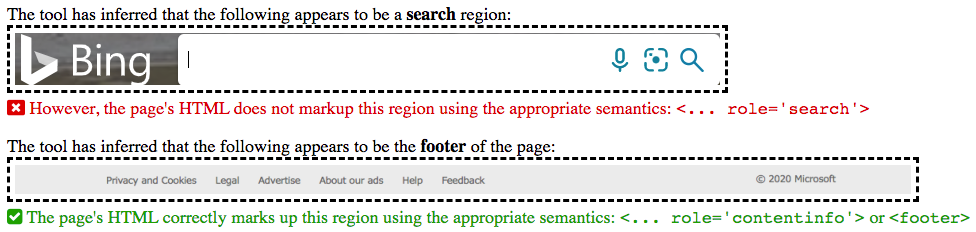
\includegraphics[scale=0.4]{accessibility_testing/figures/output-sample.png}
	\caption{Sample of the generated accessibility report.}
	\label{fig:output}
\end{figure*}


\subsection{RQ2: Accessibility Failures Detection}
While the previous question examined how accurate 
the inferred semantic groupings and roles are, 
this RQ evaluates to what extent the inferred information 
can be used to reliably detect accessibility failures.

\hl{Due to the absence of ground truth data that lists the 
actual failures per subject, 
we evaluate this RQ in two complementary ways: 
1) using a fault injection experiment, 
and 2) evaluating the output on a large number 
of real-world subjects in the wild. 
Each evaluation is independent and separate from the other. 
The rationale for using these two complementary experiments is as follows. 
In the fault injection experiment (as will be explained in \mbox{\cref{subsec:faultinjec}}), 
existing semantic markups (if any) 
are removed. This simulates an accessibility fault since, by definition, 
an accessibility fault is the \emph{absence} of required markup. 
Subsequently, a check is made whether the tool is able to detect the absent markup 
and therefore detect the fault. 
The benefit of this experiment is that it allows automated evaluation 
without a subjective assessment. In other words, it creates a partial 
ground truth data from page developers' own tagging of roles. 
The drawback, however, is that it is only a \emph{lower bound} 
of the actual accuracy, since it says nothing about other possible 
role faults that have not been injected 
(i.e., due to the absence of some roles from the original markup itself). 
For this reason, we supplement the fault injection experiment 
with a manual item-by-item evaluation of the inferred roles  
in order to evaluate all true/false positive and negative results.
We describe each approach in the following subsections. 
We emphasize that the two experiments, fault injection and direct evaluation, 
are separate and independent of each other. That is, whereas the subjects are injected with faults in the first experiment, all subjects are used in their original form 
for the second experiment. }

\begin{table}[t]
    \caption{Precision and recall of grouping and role inference. Highlighted numbers are the minimum and maximum values in each column.}
    \label{tbl:rq1}
  	\centering
    \begin{tabularx}{0.87\textwidth}{lrrrrrr}
                                   & \multicolumn{3}{c}{\textbf{Grouping inference}}                                                                                                  & \multicolumn{3}{c}{\textbf{Role inference}}                                                                                                      \\ 
    \multicolumn{1}{c}{\textbf{Subject}} & \multicolumn{1}{c}{\textbf{Prec.}}               & \multicolumn{1}{c}{\textbf{Recall}}                  & \multicolumn{1}{c}{\textbf{F-1}}               & \multicolumn{1}{c}{\textbf{Prec.}}               & \multicolumn{1}{c}{\textbf{Recall}}                  & \multicolumn{1}{c}{\textbf{F-1}}               \\  \hline
    wikipedia.org                              & 94\%                                        & 89\%                                        & 91\%                                        & 91\%                                        & 91\%                                        & 91\%                                        \\
    google.com                              & 88\%                                        & 85\%                                        & 87\%                                        & 86\%                                        & 81\%                                        & 83\%                                        \\
    amazon.com                              & 92\%                                        & 87\%                                        & 89\%                                        & \cellcolor[HTML]{DCDCDC}{\textbf{83\%}} & \cellcolor[HTML]{DCDCDC}{\textbf{79\%}} & \cellcolor[HTML]{DCDCDC}{\textbf{81\%}} \\
    stackoverflow.com                              & 91\%                                        & 94\%                                        & 92\%                                        & 91\%                                        & 81\%                                        & 86\%                                        \\
    medium.com                              & 96\%                                        & 94\%                                        & \cellcolor[HTML]{DCDCDC}{\textbf{95\%}} & 94\%                                        & \cellcolor[HTML]{DCDCDC}{\textbf{99\%}} & 96\%                                        \\
    khanacademy.org                              & 92\%                                        & \cellcolor[HTML]{DCDCDC}{\textbf{98\%}} & 95\%                                        & 96\%                                        & 89\%                                        & 93\%                                        \\
    imdb.com                              & \cellcolor[HTML]{DCDCDC}{\textbf{71\%}} & 86\%                                        & 78\%                                        & 92\%                                        & 96\%                                        & 94\%                                        \\
    cnn.com                               & \cellcolor[HTML]{DCDCDC}{\textbf{97\%}} & 92\%                                        & 95\%                                        & \cellcolor[HTML]{DCDCDC}{\textbf{97\%}} & 97\%                                        & \cellcolor[HTML]{DCDCDC}{\textbf{97\%}} \\
    rt.com                              & 92\%                                        & \cellcolor[HTML]{DCDCDC}{\textbf{60\%}} & \cellcolor[HTML]{DCDCDC}{\textbf{72\%}} & 94\%                                        & 90\%                                        & 92\%                                        \\
    booking.com                             & 92\%                                        & 73\%                                        & 81\%                                        & 93\%                                        & 89\%                                        & 91\%                                        \\ \hline
    \textbf{Average}               & \textbf{90\%}                               & \textbf{85\%}                               & \textbf{87\%}                               & \textbf{91\%}                               & \textbf{89\%}                               & \textbf{90\%}               \\               
    \end{tabularx}
    \vspace{-0.25cm}

\end{table}

\header{Subjects} We conducted the experiments in this RQ 
on a total of 30 real-world subjects. 
The subjects were collected in two ways. 
The first half of subjects were randomly selected 
from the Moz Top 500 most popular websites as in RQ1. 
The second half of subjects were obtained from Discuvver.com, 
which is a service that returns a random 
website from the internet.

% \begin{table}[]
\begin{table}%[t]
    \caption{Results of detecting fault injections.}
    \label{tbl:rq2}
    \centering
    \begin{tabular}{lrrr}
    \hline
                      & \multicolumn{1}{l}{}                                                    & \multicolumn{2}{c}{\textbf{\# Detected faults}}                                                                                                                                   \\ \cline{3-4} 
    \textbf{Subject}  & \textbf{\begin{tabular}[c]{@{}r@{}}Total \# \\ injections\end{tabular}} & \multicolumn{1}{c}{\textbf{\begin{tabular}[c]{@{}c@{}}proposed\\ approach\end{tabular}}} & \multicolumn{1}{c}{\textbf{\begin{tabular}[c]{@{}c@{}}baseline\\ \end{tabular}}} \\ \hline
    bing.com          & 1                                                                       & 1                                                                                        & 0                                                                                      \\
    youtube.com       & 3                                                                       & 3                                                                                        & 0                                                                                      \\
    google.com        & 4                                                                       & 3                                                                                        & 0                                                                                      \\
    microsoft.com     & 7                                                                       & 5                                                                                        & 0                                                                                      \\
    bbc.com           & 5                                                                       & 3                                                                                        & 0                                                                                      \\
    amazon.com        & 4                                                                       & 3                                                                                        & 0                                                                                      \\
    medium.com        & N/A                                                                     &                                                                                          &                                                                                        \\
    yahoo.com         & 3                                                                       & 1                                                                                        & 0                                                                                      \\
    live.com          & 4                                                                       & 4                                                                                        & 0                                                                                      \\
    paypal.com        & 2                                                                       & 1                                                                                        & 0                                                                                      \\
    blogger.com       & 2                                                                       & 2                                                                                        & 1                                                                                      \\
    netflix.com       & N/A                                                                     &                                                                                          &                                                                                        \\
    stackoverflow.com & 3                                                                       & 3                                                                                        & 0                                                                                      \\
    imdb.com          & 4                                                                       & 3                                                                                        & 0                                                                                      \\
    walmart.com       & 3                                                                       & 2                                                                                        & 0                                                                                      \\ \hline
    fuelly.com        & 1                                                                       & 1                                                                                        & 0                                                                                      \\
    typing.com        & 3                                                                       & 2                                                                                        & 0                                                                                      \\
    iconpacks.net     & 2                                                                       & 2                                                                                        & 0                                                                                      \\
    expatistan.com    & N/A                                                                     &                                                                                          &                                                                                        \\
    memrise.com       & N/A                                                                     &                                                                                          &                                                                                        \\
    retrevo.com       & 3                                                                       & 3                                                                                        & 0                                                                                      \\
    startupstash.com  & 4                                                                       & 3                                                                                        & 0                                                                                      \\
    eatthismuch.com   & 1                                                                       & 0                                                                                        & 0                                                                                      \\
    kdl.org           & 3                                                                       & 2                                                                                        & 0                                                                                      \\
    getpocket.com     & 2                                                                       & 2                                                                                        & 0                                                                                      \\
    retailmenot.com   & 3                                                                       & 3                                                                                        & 0                                                                                      \\
    mailinator.com    & N/A                                                                     &                                                                                          &                                                                                        \\
    myfridgefood.com  & 1                                                                       & 0                                                                                        & 0                                                                                      \\
    joinhoney.com     & 2                                                                       & 2                                                                                        & 0                                                                                      \\
    bannereasy.com    & 1                                                                       & 1                                                                                        & 0                                                                                      \\ \hline
    \textbf{Total}    & 71                                                                      & \textbf{77.5\%}                                                                          & \textbf{1.4\%}                                                                        
    \end{tabular}
    \end{table}




% \begin{table}[t]
%     \caption{Results of detecting fault injections.}
%     \label{tbl:rq2}
%     \centering
%     % \begin{tabular}{0.48\textwidth}{cccc}
%     \begin{threeparttable}
%     \bgroup 
%     \begin{tabularx}{0.43\textwidth}{lrrr}
%     \hline
%     \textbf{Subject} & \begin{tabular}[c]{@{}c@{}}\textbf{Total \#} \\ \textbf{injections}\end{tabular} & \begin{tabular}[c]{@{}c@{}}\textbf{\# Detected}\\ \textbf{faults}\end{tabular} & \begin{tabular}[c]{@{}c@{}}\textbf{\# Undetected}\\ \textbf{faults}\end{tabular} \\ \hline
%     bing.com            & 1        & 1       & 0             \\
%     youtube.com         & 3        & 3       & 0             \\
%     google.com          & 4        & 3       & 1             \\
%     microsoft.com       & 7        & 5       & 2             \\
%     bbc.com             & 5        & 3       & 2             \\
%     amazon.com          & 4        & 3       & 1             \\
%     medium.com          & N/A      &         &               \\   
%     yahoo.com           & 3        & 1       & 2             \\
%     live.com            & 4        & 4       & 0             \\
%     paypal.com          & 2        & 1       & 1             \\
%     blogger.com         & 2        & 2       & 0             \\
%     netflix.com         & N/A      &         &               \\   
%     stackoverflow.com   & 3        & 3       & 0             \\
%     imdb.com            & 4        & 3       & 1             \\
%     walmart.com         & 3        & 2       & 1             \\ \hline 
%     fuelly.com          & 1        & 1       & 0             \\
%     typing.com          & 3        & 2       & 1             \\
%     iconpacks.net       & 2        & 2       & 0             \\
%     expatistan.com      & N/A      &         &               \\    
%     memrise.com         & N/A      &         &               \\  
%     retrevo.com         & 3        & 3       & 0             \\
%     startupstash.com    & 4        & 3       & 1             \\
%     eatthismuch.com     & 1        & 0       & 1             \\
%     kdl.org             & 3        & 2       & 1             \\
%     getpocket.com       & 2        & 2       & 0             \\
%     retailmenot.com     & 3        & 3       & 0             \\
%     mailinator.com      & N/A      &         &               \\      
%     myfridgefood.com    & 1        & 0       & 1             \\
%     joinhoney.com       & 2        & 2       & 0             \\
%     bannereasy          & 1        & 1       & 0             \\ \hline
  
%     \textbf{Total}      & 71       & \textbf{77.5\%}      & \textbf{22.5\%} 
%     % \end{tabular}
%     \end{tabularx}
%     \egroup
%     %% This how it should be used in a cell: \multicolumn{3}{c}{N/A\tnote\textdagger}
%     % \begin{tablenotes}
%     %     \item[\textdagger] Faults could not be injected. Please refer to \cref{subsec:rq2-results} for details.
%     % \end{tablenotes}
% \end{threeparttable}
% \vspace{-0.25cm}
% \end{table}





\subsubsection{Fault injection}\label{subsec:faultinjec}
For the fault injection experiment, we inject a random fault in the markup of each subject, and 
assess if \toolname was able to detect the fault. 
We recall from \Cref{subsec:aria-roles} that a web page 
is deemed inaccessible if there is an \emph{absence} of semantic roles. That is, the developer did not add the necessary semantic markup to the page. Our goal is thus to simulate this behavior by \emph{removing} all existing semantic markups on the page, and therefore create a new page as if the developer had not included the necessary semantic markup, and then check whether our approach can re-detect them. Such markup omission, by definition, is what makes web pages inaccessible, 
and is therefore the only meaningful fault type. 
In other words, any mutation of the markup is effectively a markup omission, 
since the exact expected semantic role would become absent from the markup. Due to the absence of ground truth information, 
the next best unbiased option we have is to assume that if a developer has taken the time to manually identify the role of each region, then we take that to be correct. 
We also note that misspelled attribute values are also effectively markup omissions. 
For instance, suppose that a region should have been marked as a navigation region. 
Whether the \code{navigation} role was completely absent from the markup, 
or was misspelled (i.e., \code{ngavoitn}), both cases are still effectively markup omissions.

We now describe the injection process.
First, we load the subject in an instrumented browser (i.e., via Selenium). 
We then remove all semantic markups on the page 
(i.e., landmark \code{role}s). 
We then apply \toolname on the subject and collect the output.  
If after the fault injection (i.e., removal of \code{role}s) 
\toolname was able to indicate that there should be a semantic \code{role} (per each removed markup), 
we conclude that the injected fault has been caught. 
Otherwise, the fault was not detected. 


\header{Baseline}
In order to have a more thorough evaluation, 
we included a baseline in our experiments. 
We could have just reported the results on their own, but 
adding a baseline offers some perspective on how relatively 
better the approach is. 
However, since there are no existing tools that perform 
semantic checking, 
our baseline consists of a simple random selection process. 
In this process, random regions from the page 
are selected. Next, a random semantic role is 
assigned to each randomly selected region. 
This set of semantic regions and their semantic roles 
is then taken to be the baseline.  

\header{Results and Discussion}\label{subsec:rq2-results}
\Cref{tbl:rq2} shows the results of evaluating the fault 
injection experiment. 
The first column shows the total number of fault injections performed on 
each subject. 
We recall that this first column is not a number we chose; 
it is rather the total number of injections that were \emph{possible}, 
since the faults are removals of existing semantic markup. 
The second column shows the number of injected faults that 
were successfully detected by, whereas the third column shows the 
number of injected faults that the tool has failed to detect. 
The last row sums up the results across all subjects.

The main result of the evaluation is that \toolname has detected, 
on average, around 77.5\% of the injected faults. 
While this performance is relatively good, 
given that this sort of analysis hasn't been automated so far, 
we do note this is only a lower bound of the actual accessibility 
failure detection ability, since it says nothing about other possible 
failures that have not been injected 
(e.g., where the original markup itself did not include certain semantic roles). 

In certain subjects in \Cref{tbl:rq2}, marked with ``N/A'', the fault 
injection process was not possible. 
This was because the subject's markup did not contain any of the landmark semantic roles, 
and therefore it was not possible to remove them and check if our tool 
was able to detect them back. 
Despite some of these subjects being top 100 websites, 
the lack of such markup in the subject is an example that illustrates the need for effective 
and automated accessibility testing.

\subsubsection{Direct output evaluation}
In this step, we manually evaluate the output on a large number 
of real-world subjects in the wild.
First, we loaded each test subject in an instrumented web browser (i.e., via Selenium). 
Page popups or notifications, if any, were closed. 
Next, we applied \toolname on the subject and collected the generated 
output (as shown in \Cref{fig:output}).  
We then categorized each item in the report into one of the following:
\textit{True positive:} 
This represents a true accessibility failure. 
This category holds whenever the tool has reported the absence of 
a correct semantic role that is indeed missing from markup, 
and therefore the reported failure is true.   
\textit{False positive:}
This is a false accessibility failure.
In this case the tool has either reported an incorrect semantic 
role or the role is already in the markup 
but was falsely flagged as missing, and therefore 
the reported failure is false.
\textit{False negative:}
This case is a false accessibility \emph{pass} 
(not failure, as in the two previous cases).
This represents cases where a semantic role should have been included the markup, as determined by manual visual examination of the page, but the approach did not report an accessibility failure. For instance, the page has a search region but the approach did not 
report that role. 
\textit{True negative:}
This corresponds to true accessibility pass.  
This represents cases where a role is actually semantically not present 
on the page, and the tool did not report a failure.
This also corresponds to cases where a semantic role is present in the markup, 
and the tool has reported that the markup is conforming to the inferred semantic role.  

% \caption{Direct evaluation of accessibility failure detection on 30 real-world subjects in the wild.}
% \label{tbl:rq2-run}


% \begin{table}[]

%     \begin{tabular}{lrrrr}
%     \hline
%     \textbf{Subject}  & \textbf{TP}   & \textbf{FP}    & \textbf{TN}   & \textbf{FN}  \\ \hline
%     bing.com          & 4             & 0              & 1             & 0            \\
%     youtube.com       & 0             & 0              & 4             & 0            \\
%     google.com        & 2             & 2              & 3             & 0            \\
%     microsoft.com     & 2             & 1              & 10            & 0            \\
%     bbc.com           & 2             & 2              & 2             & 2            \\
%     amazon.com        & 4             & 0              & 7             & 0            \\
%     medium.com        & 4             & 0              & 1             & 0            \\
%     yahoo.com         & 1             & 0              & 1             & 3            \\
%     live.com          & 2             & 0              & 4             & 0            \\
%     paypal.com        & 3             & 0              & 2             & 0            \\
%     blogger.com       & 1             & 0              & 3             & 1            \\
%     netflix.com       & 2             & 0              & 1             & 1            \\
%     stackoverflow.com & 3             & 0              & 6             & 0            \\
%     imdb.com          & 2             & 2              & 3             & 0            \\
%     walmart.com       & 6             & 0              & 2             & 1            \\ \hline
%     fuelly.com        & 3             & 0              & 2             & 0            \\
%     typing.com        & 2             & 1              & 3             & 2            \\
%     iconpacks.net     & 3             & 0              & 1             & 1            \\
%     expatistan.com    & 2             & 3              & 1             & 0            \\
%     memrise.com       & 4             & 1              & 2             & 0            \\
%     retrevo.com       & 2             & 0              & 3             & 0            \\
%     startupstash.com  & 1             & 0              & 4             & 0            \\
%     eatthismuch.com   & 6             & 0              & 1             & 0            \\
%     kdl.org           & 3             & 1              & 2             & 1            \\
%     getpocket.com     & 2             & 0              & 3             & 0            \\
%     retailmenot.com   & 5             & 0              & 3             & 0            \\
%     mailinator.com    & 2             & 1              & 1             & 0            \\
%     myfridgefood.com  & 2             & 1              & 1             & 1            \\
%     joinhoney.com     & 3             & 0              & 3             & 0            \\
%     bannereasy.com    & 4             & 0              & 2             & 0            \\ \hline
%                                    &               &                &               &              \\
%                                    & \textbf{Acc.} & \textbf{Prec.} & \textbf{Rec.} & \textbf{F-1} \\
%                                    & 85.4\%        & 84.5\%         & 86.3\%        & 85.4\%      
%     \end{tabular}
%     \end{table}

\newcommand{\PreserveBackslash}[1]{\let\temp=\\#1\let\\=\temp}
\newcolumntype{C}[1]{>{\PreserveBackslash\centering}p{#1}}
\newcolumntype{R}[1]{>{\PreserveBackslash\raggedleft}p{#1}}
\newcolumntype{L}[1]{>{\PreserveBackslash\raggedright}p{#1}}


%\begin{table*}[ht]
\begin{sidewaystable}
    \caption{Direct evaluation of accessibility failure detection 
    on 30 real-world subjects. 
    % For comparison, the output of the state-of-the-art (SortSite) is included.
    }
    \label{tbl:rq2-run}
    \centering
    % \begin{tabular}{lrrrrrr}
    % \begin{tabular}{p{1.8cm}p{0.01cm}p{0.01cm}p{0.01cm}p{0.01cm}p{1cm}p{1cm}}
    \begin{tabularx}{0.85\textwidth}{p{2.5cm}R{0.4cm}R{0.4cm}R{0.4cm}R{0.4cm}L{1.4cm}R{1.4cm}R{0.4cm}R{0.4cm}R{0.4cm}R{0.4cm}}
    \hline
                      & \multicolumn{4}{c|}{\textbf{Proposed approach}}                                                                                               & \multicolumn{2}{C{3.2cm}|}{\textbf{SortSite}}                                                                                                                                                                & \multicolumn{4}{c}{\textbf{Baseline}}                                                                                                                               \\
    \textbf{Subject}  & \multicolumn{1}{c}{\textbf{TP}} & \multicolumn{1}{c}{\textbf{FP}} & \multicolumn{1}{c}{\textbf{TN}} & \multicolumn{1}{C{0.3cm}|}{\textbf{FN}} & \multicolumn{1}{C{0.9cm}}{\textbf{\begin{tabular}[c]{@{}c@{}}semantic \\ issues\end{tabular}}} & \multicolumn{1}{C{0.6cm}|}{\textbf{\begin{tabular}[c]{@{}c@{}}syntactic \\ issues\end{tabular}}}            & \multicolumn{1}{c}{\textbf{TP}} & \multicolumn{1}{c}{\textbf{FP}} & \multicolumn{1}{c}{\textbf{TN}}   & \multicolumn{1}{C{0.3cm}}{\textbf{FN}}                                                          \\ \hline
    bing.com          & 4                               & 0                               & 1                               & \multicolumn{1}{R{0.3cm}|}{0}           & 0                                                                                       & \multicolumn{1}{R{0.3cm}|}{11}                                                                                     & 0                               & 3                               & 0                                 & 4                                                                                                                                                                                                \\
    youtube.com       & 0                               & 0                               & 4                               & \multicolumn{1}{R{0.3cm}|}{0}           & 0                                                                                       & \multicolumn{1}{R{0.3cm}|}{10}                                                                                     & 0                               & 2                               & 0                                 & 0                                                                                                                                   \\
    google.com        & 2                               & 2                               & 3                               & \multicolumn{1}{R{0.3cm}|}{0}           & 0                                                                                       & \multicolumn{1}{R{0.3cm}|}{6}                                                                                      & 0                               & 2                               & 0                                 & 2                                                                                                                                              \\
    microsoft.com     & 2                               & 1                               & 10                              & \multicolumn{1}{R{0.3cm}|}{0}           & 0                                                                                       & \multicolumn{1}{R{0.3cm}|}{10}                                                                                     & 0                               & 1                               & 0                                 & 2                                                                                                   \\
    bbc.com           & 2                               & 2                               & 2                               & \multicolumn{1}{R{0.3cm}|}{2}           & 0                                                                                       & \multicolumn{1}{R{0.3cm}|}{3}                                                                                      & 0                               & 4                               & 0                                 & 4                                                              \\
    amazon.com        & 4                               & 0                               & 7                               & \multicolumn{1}{R{0.3cm}|}{0}           & 0                                                                                       & \multicolumn{1}{R{0.3cm}|}{13}                                                                                     & 0                               & 1                               & 0                                 & 4                                                               \\
    medium.com        & 4                               & 0                               & 1                               & \multicolumn{1}{R{0.3cm}|}{0}           & 0                                                                                       & \multicolumn{1}{R{0.3cm}|}{6}                                                                                      & 0                               & 2                               & 0                                 & 4                                                               \\
    yahoo.com         & 1                               & 0                               & 1                               & \multicolumn{1}{R{0.3cm}|}{3}           & 0                                                                                       & \multicolumn{1}{R{0.3cm}|}{9}                                                                                      & 0                               & 3                               & 0                                 & 4                                                               \\
    live.com          & 2                               & 0                               & 4                               & \multicolumn{1}{R{0.3cm}|}{0}           & 0                                                                                       & \multicolumn{1}{R{0.3cm}|}{2}                                                                                      & 0                               & 3                               & 0                                 & 2                                                               \\
    paypal.com        & 3                               & 0                               & 2                               & \multicolumn{1}{R{0.3cm}|}{0}           & 0                                                                                       & \multicolumn{1}{R{0.3cm}|}{13}                                                                                     & 0                               & 2                               & 0                                 & 3                                                               \\
    blogger.com       & 1                               & 0                               & 3                               & \multicolumn{1}{R{0.3cm}|}{1}           & 0                                                                                       & \multicolumn{1}{R{0.3cm}|}{5}                                                                                      & 1                               & 2                               & 0                                 & 2                                                               \\
    netflix.com       & 2                               & 0                               & 1                               & \multicolumn{1}{R{0.3cm}|}{1}           & N/A                                                                                     & \multicolumn{1}{R{0.3cm}|}{N/A}                                                                                    & 0                               & 4                               & 0                                 & 3                                                                                                                                     \\
    stackoverflow.com & 3                               & 0                               & 6                               & \multicolumn{1}{R{0.3cm}|}{0}           & 0                                                                                       & \multicolumn{1}{R{0.3cm}|}{18}                                                                                     & 0                               & 2                               & 0                                 & 3                                                               \\
    imdb.com          & 2                               & 2                               & 3                               & \multicolumn{1}{R{0.3cm}|}{0}           & N/A                                                                                     & \multicolumn{1}{R{0.3cm}|}{N/A}                                                                                    & 0                               & 3                               & 0                                 & 2                                                                                                                                     \\
    walmart.com       & 6                               & 0                               & 2                               & \multicolumn{1}{R{0.3cm}|}{1}           & 0                                                                                       & \multicolumn{1}{R{0.3cm}|}{7}                                                                                      & 0                               & 4                               & 0                                 & 7                                                               \\ \hline
    fuelly.com        & 3                               & 0                               & 2                               & \multicolumn{1}{R{0.3cm}|}{0}           & 0                                                                                       & \multicolumn{1}{R{0.3cm}|}{12}                                                                                     & 0                               & 1                               & 0                                 & 3                                                               \\
    typing.com        & 2                               & 1                               & 3                               & \multicolumn{1}{R{0.3cm}|}{2}           & 0                                                                                       & \multicolumn{1}{R{0.3cm}|}{10}                                                                                     & 0                               & 2                               & 0                                 & 4                                                               \\
    iconpacks.net     & 3                               & 0                               & 1                               & \multicolumn{1}{R{0.3cm}|}{1}           & 0                                                                                       & \multicolumn{1}{R{0.3cm}|}{8}                                                                                      & 0                               & 4                               & 0                                 & 4                                                               \\
    expatistan.com    & 2                               & 3                               & 1                               & \multicolumn{1}{R{0.3cm}|}{0}           & 0                                                                                       & \multicolumn{1}{R{0.3cm}|}{9}                                                                                      & 0                               & 1                               & 0                                 & 2                                                               \\
    memrise.com       & 4                               & 1                               & 2                               & \multicolumn{1}{R{0.3cm}|}{0}           & 0                                                                                       & \multicolumn{1}{R{0.3cm}|}{5}                                                                                      & 0                               & 1                               & 0                                 & 4                                                               \\
    retrevo.com       & 2                               & 0                               & 3                               & \multicolumn{1}{R{0.3cm}|}{0}           & N/A                                                                                     & \multicolumn{1}{R{0.3cm}|}{N/A}                                                                                    & 0                               & 2                               & 0                                 & 2                                                                                                                                     \\
    startupstash.com  & 1                               & 0                               & 4                               & \multicolumn{1}{R{0.3cm}|}{0}           & 0                                                                                       & \multicolumn{1}{R{0.3cm}|}{12}                                                                                     & 0                               & 4                               & 0                                 & 1                                                               \\
    eatthismuch.com   & 6                               & 0                               & 1                               & \multicolumn{1}{R{0.3cm}|}{0}           & 0                                                                                       & \multicolumn{1}{R{0.3cm}|}{15}                                                                                     & 0                               & 3                               & 0                                 & 6                                                               \\
    kdl.org           & 3                               & 1                               & 2                               & \multicolumn{1}{R{0.3cm}|}{1}           & 0                                                                                       & \multicolumn{1}{R{0.3cm}|}{9}                                                                                      & 0                               & 3                               & 0                                 & 4                                                               \\
    getpocket.com     & 2                               & 0                               & 3                               & \multicolumn{1}{R{0.3cm}|}{0}           & 0                                                                                       & \multicolumn{1}{R{0.3cm}|}{7}                                                                                      & 0                               & 1                               & 0                                 & 2                                                               \\
    retailmenot.com   & 5                               & 0                               & 3                               & \multicolumn{1}{R{0.3cm}|}{0}           & 0                                                                                       & \multicolumn{1}{R{0.3cm}|}{2}                                                                                      & 0                               & 2                               & 0                                 & 5                                                               \\
    mailinator.com    & 2                               & 1                               & 1                               & \multicolumn{1}{R{0.3cm}|}{0}           & 0                                                                                       & \multicolumn{1}{R{0.3cm}|}{6}                                                                                      & 0                               & 4                               & 0                                 & 2                                                               \\
    myfridgefood.com  & 2                               & 1                               & 1                               & \multicolumn{1}{R{0.3cm}|}{1}           & 0                                                                                       & \multicolumn{1}{R{0.3cm}|}{8}                                                                                      & 0                               & 2                               & 0                                 & 3                                                               \\
    joinhoney.com     & 3                               & 0                               & 3                               & \multicolumn{1}{R{0.3cm}|}{0}           & 0                                                                                       & \multicolumn{1}{R{0.3cm}|}{7}                                                                                      & 0                               & 3                               & 0                                 & 3                                                               \\
    bannereasy.com    & 4                               & 0                               & 2                               & \multicolumn{1}{R{0.3cm}|}{0}           & 0                                                                                       & \multicolumn{1}{R{0.3cm}|}{5}                                                                                      & 0                               & 1                               & 0                                 & 4                                                               \\ \hline
                    %   & \multicolumn{1}{l}{}            & \multicolumn{1}{l}{}            & \multicolumn{1}{l}{}            & \multicolumn{1}{r|}{}             & \multicolumn{1}{l}{}                                                                    & \multicolumn{1}{l}{}                                                                     \\
                      & \multicolumn{1}{r}{\textbf{Acc.}}                   & \multicolumn{1}{r}{\textbf{Prec.}}                  & \multicolumn{1}{r}{\textbf{Rec.}}                   & \multicolumn{1}{l|}{\textbf{F1}}                     & \multicolumn{1}{r}{}                                                                    & \multicolumn{1}{r|}{}                      & \multicolumn{1}{r}{\textbf{Acc.}}                   & \multicolumn{1}{r}{\textbf{Prec.}}                  & \multicolumn{1}{r}{\textbf{Rec.}}                   & \multicolumn{1}{l}{\textbf{F1}}                                                                                                                                                                                                             \\
                      & 85.4\%                          & 84.5\%                          & 86.3\%                          & \multicolumn{1}{r|}{85.4\%}                    & \multicolumn{1}{r}{}                                                                    & \multicolumn{1}{r|}{}                                                                                        & 0.6\%                          & 1.3\%                          & 1.0\%                          & \multicolumn{1}{r}{1.2\%}                                           
    % \end{tabular}
\end{tabularx}
    \vspace{-0.25cm}
%    \end{table*}
\end{sidewaystable}


\header{Results and Discussion}\label{subsec:run-results}
\Cref{tbl:rq2-run} shows the results of the evaluation. 
Each row lists the subject, the true positive/negative and 
the false positive/negative for the subject. 
The last row shows the accuracy, precision, 
recall, and the F-1 measure. 

The values of the accuracy, precision, and recall 
are between 84\% and 86\%, indicating a relatively good 
performance. The true positive column represents the 
true accessibility failures that are indeed present in the subjects. 
This certainly does not cover all possible accessibility failures, 
but rather the subset of accessibility issues that we focus on in this 
work (i.e., the semantic roles).
The true negative column can be thought of as the number of cases 
where the markup of the subject is ``in agreement'' 
with the tool's output.  
In the median, two true accessibility failures were detected per subject, 
and two inferred semantic roles per subject were in agreement with what has been 
expressed in the markup. 
For the second half of subjects in \Cref{tbl:rq2-run} (i.e., the random sites), 
60\% have used semantic roles. In contrast, for the subset of top websites 
(i.e., the first half of subjects), 
74\% have used semantic roles.
40\% of the random websites did not use any semantic roles, compared 
to 26\% of the top websites.    
This observation is expected since top sites are more likely 
to have more resources to create better products. 
The average execution runtime was 17 seconds.

We then investigated the reasons behind the false positives and negatives. 
One common reason is erroneous inference of navigation roles. 
This occurred, for instance, for a region that consisted of weather forecast 
for the next few days. From the perspective of our inference procedure, 
this looked like a navigation area since it had a group of links that were 
coherent in content and presentation (in the sense described in \Cref{sec:role-inf}).
Accordingly, it was falsely indicated as a navigation (i.e., a false positive), and therefore resulted 
in a false accessibility failure. Another reason involves missing footer roles 
that should have been reported. This occurred, for instance, 
for a region that was not recognized by the semantic grouping stage, and therefore 
no role was able to be inferred for it.

For comparison, \Cref{tbl:rq2-run} also includes an evaluation 
of SortSite\footnote{https://www.powermapper.com/products/sortsite/}, 
which is the best performing state-of-the-art 
accessibility testing tool~\cite{ukgov:audit:2018}. 
As mentioned in the introduction, SortSite and other state-of-the-art tools 
only perform syntactic checks and is therefore 
unable to detect the semantic issues 
that are the focus of this work. Accordingly, we run 
an evaluation that verifies this empirically. 
Each subject is fed to SortSite, and the output report is saved. 
Each reported failure is then 
categorized as either a syntactic issue or a semantic issue. 
We recall that, as discussed in \Cref{subsec:syncheckers}, 
a syntactic issue is any failure that only checks the syntax 
of the HTML. Examples include checks like (``each \code{a} 
element must contain non-empty text''), or (``\code{input} must not 
appear as a descendant of \code{a}''). 
These are direct checks that are only concerned with syntax. 
Compare this, for instance, with the reported failure shown in \Cref{fig:output}. 
Here, the failure is \emph{semantic} in nature. That is, the failure 
is not an application of some syntactic rule. Rather, 
the failure is reported because the markup does not conform to how the 
page \emph{is semantically perceived} from a visual perspective, not 
because it didn't conform to a predetermined syntactic rule. 

From \Cref{tbl:rq2-run}, we observe that SortSite was able to 
find many syntactic issues 
(rows with N/A are cases were the tool was unable to load the subject). 
However, it did not detect any of the semantic issues. 
This is expected, as the rationale for this work was the observation 
that the state-of-the-art only conduct syntactic checks, which cannot 
detect the more important and widely used semantic information. 

\subsubsection{Future work}
In this work, we focused on an important subset of accessibility requirements, 
which are the semantic roles as discussed in \ref{header:targeted-roles}. 
Therefore, as expected, our approach 
can not cover all possible accessibility requirements. 
This leaves open a number of avenues 
for future work to address other accessibility requirements, each of which would require 
a novel technique to address. 
The variations in the semantics of various accessibility requirements and the lack of approaches 
to address them, mainly due to the difficulty of performing high-level semantic analysis, 
presents a rich and fertile ground to conduct research, which has received little attention 
from the software engineering research community as discussed in the introduction. 
For future work, we believe it will be a fruitful and interesting pursuit for the research 
community to explore some of these other accessibility requirements.

\subsubsection{Threats to validity}
We chose test subjects (i.e., web sites) randomly from the Internet
with the mentioned criteria in \Cref{sec:evaluation},
to avoid any selection bias.
Plus, the participants were selected to be highly qualified 
evaluators at the crowdsourcing platform, 
mitigating the threats to the internal validity of the study.
The subjects are diverse and complex enough
to be representative of real-world scenarios,
mitigating the external validity of the study by making the results generalizable.
To make the study replicable, we made available online a link to 
our \toolname tool and the anonymized participants' responses~\cite{tool-and-data}.
